% !TEX encoding = UTF-8 Unicode
% !TEX program = xelatex

\documentclass{article}
	\usepackage[paper width=11in,paper height=11in,margin=.25in]{geometry}
	\usepackage{xeCJK}
		\setmainfont{SourceCodePro-Regular}
		\setCJKmainfont{NotoSansTC-Regular}
	\usepackage{tikz}
	\usepackage{tikz-3dplot}
	\usepackage{listings}
\begin{document}

\lstset{
	language=[latex]tex,tabsize=4,
	moredelim=*[s][\itshape]{$}{$},
	moredelim=*[s][\color{red!40!.}]{(}{)},
	moredelim=*[s][\color{green!30!.}]{[}{]},
	backgroundcolor=\color{blue!5},
	commentstyle=\color{.!80}\itshape,
	texcsstyle=*\color{blue!40!.},
	moretexcs={
		foreach,
		tdplotsetmaincoords,pgfpointxyz,
		pgfmathsetmacro,pgfmathtruncatemacro,pgfmathsetlength,
		pgf@x,pgf@y,rcarot,rcbrot,rccrot,pgftemp@x,pgftemp@y,pgftemp@z
	},
	deletetexcs={h,a,b,c},
}
%%%%%%%%%%%%%%%%%%%%%%%%%%%%%%%%%%%%%%%%%%%%%%%%%%%%%%%%%%%%%%%%%%%%%%%%%%%%%%%%
\begin{lstlisting}%%%%%%%%%%%%%%%%%%%%%%%%%%%%%%%%%%%%%%%%%%%%%%%%%%%%%%%%%%%%%%

% !TEX encoding = UTF-8 Unicode
% !TEX program = pdflatex
\documentclass[border = 1cm, tikz]{standalone}\usepackage{tikz-3dplot}
\begin{document}
	\makeatletter\let\oldpointxyz\pgfpointxyz\def\pgfpointxyz#1#2#3{% perspective projection
		\oldpointxyz{#1-\camerax}{#2-\cameray}{#3-\cameraz}%%% (x,y,z) is camera center
		\pgfmathsetmacro\depth{\rcarot*\pgftemp@x+\rcbrot*\pgftemp@y+\rccrot*\pgftemp@z}
		\pgfmathsetlength\pgf@x{\pgf@x*\cameras/(\camerad-\depth)}%%% camera scale and distance
		\pgfmathsetlength\pgf@y{\pgf@y*\cameras/(\camerad-\depth)}}\makeatother
	\tdplotsetmaincoords{50}{120}%視角
	\def\camerax{0}\def\cameray{0}\def\cameraz{8}\def\camerad{40}\def\cameras{20}%相機中心、距離、倍率
	\begin{tikzpicture}[tdplot_main_coords]
		\def\block(#1,#2,#3)[#4,#5,#6];{
			\pgfmathsetmacro\a{#1}\pgfmathsetmacro\A{\a+1}
			\pgfmathsetmacro\b{#2}\pgfmathsetmacro\B{\b+1}
			\pgfmathsetmacro\c{#3}\pgfmathsetmacro\C{\c+1}
			\pgfmathsetmacro\rnd{rnd*10}
			\fill[.!\rnd!#4](\a,\b,\C)--(\A,\b,\C)--(\A,\B,\C)--(\a,\B,\C)--cycle;%上蓋
			\fill[.!\rnd!#5](\A,\b,\c)--(\A,\B,\c)--(\A,\B,\C)--(\A,\b,\C)--cycle;%左側面
			\fill[.!\rnd!#6](\a,\B,\c)--(\a,\B,\C)--(\A,\B,\C)--(\A,\B,\c)--cycle;%右側面
		}
		\colorlet{g1}{green!80!.}\colorlet{d1}{brown!80!.}%\colorlet{s1}{gray!80!.}%上色
		\colorlet{g2}{green!65!.}\colorlet{d2}{brown!65!.}%\colorlet{s2}{gray!65!.}%左色
		\colorlet{g3}{green!50!.}\colorlet{d3}{brown!50!.}%\colorlet{s3}{gray!50!.}%右色
		\def\grass(#1,#2,#3){\block(#1,#2,#3)[g1,g2,g3]}%草方塊
		\def\dirt(#1,#2,#3){\block(#1,#2,#3)[d1,d2,d3]}%土方塊
		%\def\stone(#1,#2,#3){\block(#1,#2,#3)[s1,s2,s3]}%石方塊
		\foreach \x in {-15, ..., 15}{
			\foreach \y in {-15, ..., 15}{
				\pgfmathtruncatemacro\radi{sqrt((\x)^2 + (\y)^2)}%限制半徑
				\ifdim\radi pt < 15pt%方圓 15 公尺
					\pgfmathtruncatemacro\Z{sin(\x*31-\y*19) * 3.5 +
					                        sin(\x*17+\y*26) * 2 + 5.5}%地形函數
					%\foreach \z in {0, ..., \Z}{\stone(\x,\y,\z);}%堆石頭
					\dirt(\x,\y,\Z);%放土
					\dirt(\x,\y,\Z+1);%放土
					\grass(\x,\y,\Z+2);%放草
				\fi
			}
		}
	\end{tikzpicture}
\end{document}

\end{lstlisting}%%%%%%%%%%%%%%%%%%%%%%%%%%%%%%%%%%%%%%%%%%%%%%%%%%%%%%%%%%%%%%%%
%%%%%%%%%%%%%%%%%%%%%%%%%%%%%%%%%%%%%%%%%%%%%%%%%%%%%%%%%%%%%%%%%%%%%%%%%%%%%%%%

\tikz[remember picture,overlay]\path(0,0)(17,-1.7)node{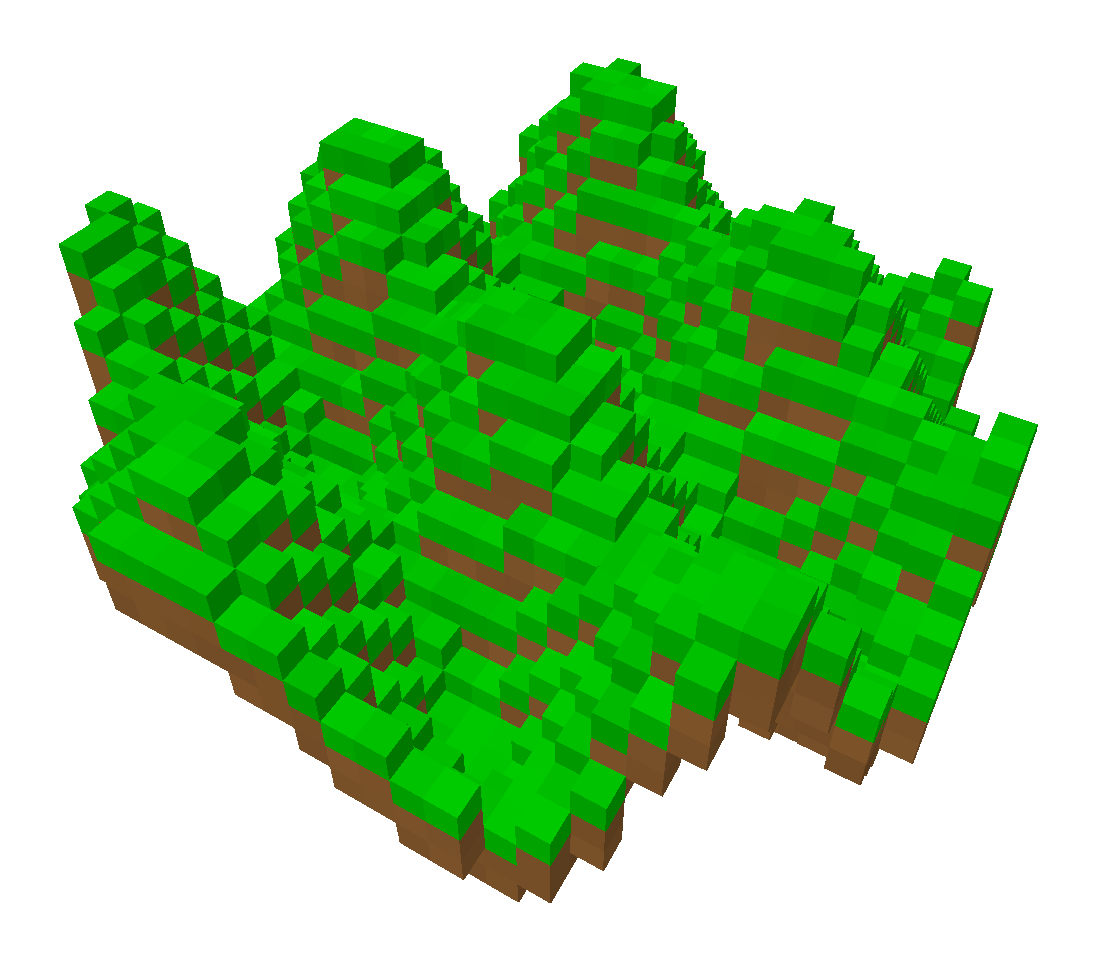
\includegraphics{minecraft.pdf}};

\end{document}